\documentclass[conference]{IEEEtran}

\usepackage{cite}
\usepackage{amsmath,amssymb,amsfonts}
\usepackage{graphicx}
\usepackage{booktabs}
\usepackage{array}
\usepackage{url}
\usepackage{xcolor}

\title{Notes on Linear Regression}

\author{
\IEEEauthorblockN{Luis Mendez}
}

\begin{document}
\maketitle

\section{Assumptions of Linear Regression}
\begin{itemize}
    \item Linearity: The relationship between the independent and dependent variable is linear.
    \item Independence: The residuals (errors) are independent of each other.
    \item Homoscedasticity: The residuals have constant variance at every level of the independent variable.
    \item Normality: The residuals are normally distributed.
    \item Multivariate Normality: The independent variables are normally distributed (for multiple regression).
    \item No Multicollinearity: The independent variables are not highly correlated with each other.
\end{itemize}
\begin{figure}[ht]
    \centering
    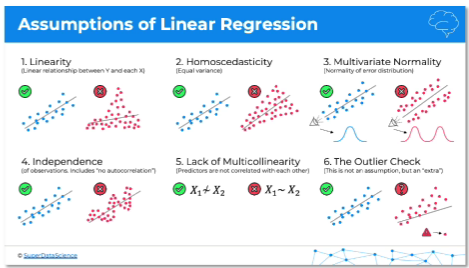
\includegraphics[width=0.8\linewidth]{linear_regression_assumptions.png}
\end{figure}

\section{Building a model}
\begin{itemize}
    \item Define the problem and collect data.
    \item Preprocess the data (handle missing values, encode categorical variables, etc.).
    \item Split the data into training and testing sets.
    \item Train the linear regression model on the training data.
    \item Evaluate the model using metrics such as Mean Absolute Error (MAE), Mean Squared Error (MSE), or R-squared on the testing data.
    \item Interpret the coefficients to understand the relationship between independent and dependent variables.
\end{itemize}

\end{document}
